\let\negmedspace\undefined
\let\negthickspace\undefined
\documentclass[journal,12pt,onecolumn]{IEEEtran}
\usepackage{cite}
\usepackage{amsmath,amssymb,amsfonts,amsthm}
\usepackage{amsmath}
\usepackage{algorithmic}
\usepackage{graphicx}
\usepackage{textcomp}
\usepackage{xcolor}
\usepackage{txfonts}
\usepackage{listings}
\usepackage{multicol}
\usepackage{enumitem}
\usepackage{mathtools}
\usepackage{gensymb}
\usepackage{comment}
\usepackage[breaklinks=true]{hyperref}
\usepackage{tkz-euclide} 
\usepackage{listings}
\usepackage{gvv}                                        
\usepackage[latin1]{inputenc}                                
\usepackage{color}                                            
\usepackage{array}                                            
\usepackage{longtable}                                       
\usepackage{calc}                                             
\usepackage{multirow}                                         
\usepackage{hhline}                                           
\usepackage{ifthen}                                           
\usepackage{lscape}
\usepackage{tabularx}
\usepackage{array}
\usepackage{float}
\usepackage{tikz}
\usepackage{multicol}
\usepackage{circuitikz}
\usetikzlibrary{patterns}
\newtheorem{theorem}{Theorem}[section]
\newtheorem{problem}{Problem}
\newtheorem{proposition}{Proposition}[section]
\newtheorem{lemma}{Lemma}[section]
\newtheorem{corollary}[theorem]{Corollary}
\newtheorem{example}{Example}[section]
\newtheorem{definition}[problem]{Definition}
\newcommand{\BEQA}{\begin{eqnarray}}
\newcommand{\EEQA}{\end{eqnarray}}
\newcommand{\define}{\stackrel{\triangle}{=}}
\theoremstyle{remark}
\newtheorem{rem}{Remark}

\begin{document}

\bibliographystyle{IEEEtran}
\vspace{3cm}

\title{2021-AE}
\author{EE24BTECH11020 -  Ellanti Rohith}
\maketitle

\renewcommand{\thefigure}{\theenumi}
\renewcommand{\thetable}{\theenumi}
\begin{enumerate}
  \item The figure shows schematics of wave patterns at the exit of nozzles A and B operating at different pressure ratios.

 \begin{multicols}{2}
    \begin{enumerate}
 \item 
\begin{tikzpicture}
            \fill[gray] (0,0) -- (-0.5,1) -- (1,1) -- (1.5,0)-- cycle;
              \fill[gray] (0,0) -- (-0.5,-1) -- (1,-1) -- (1.5,0) -- cycle;
        \end{tikzpicture}        
        \item 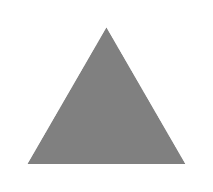
\begin{tikzpicture}
            \fill[gray] (0,0) -- (1,1.73) -- (2,0) -- cycle;
        \end{tikzpicture}
       \item 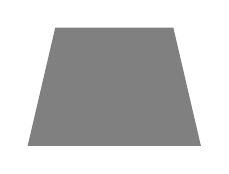
\begin{tikzpicture}
            \fill[gray] (0,0) -- (2.2,0) -- (1.85,1.5) -- (0.35,1.5) -- cycle; 
            
        \end{tikzpicture}
        \item  
\begin{tikzpicture}
            \fill[gray] (0,0) rectangle (2,2);
        \end{tikzpicture}
        
        
    \end{enumerate}
    \end{multicols}

\begin{figure}[!ht]
\centering
\resizebox{0.3\textwidth}{!}{%
\begin{circuitikz}
\tikzstyle{every node}=[font=\large]
\draw [ line width=1.2pt](3.75,11.75) to[short] (3.75,6.75);
\draw [ line width=1.2pt](3.75,6.75) to[short] (8.75,6.75);
\draw [ line width=1.2pt](8.75,11.75) to[short] (8.75,6.75);
\draw [ line width=1.2pt](3.75,11.75) to[short] (8.75,11.75);
\draw [line width=1.2pt, dashed] (5,11.75) -- (5,6.75);
\draw [line width=1.2pt, dashed] (7.5,11.75) -- (7.5,6.75);
\draw [line width=1.2pt, dashed] (3.75,10.5) -- (8.75,10.5);
\draw [line width=1.2pt, dashed] (3.75,8) -- (8.75,8);
\draw [ line width=1.2pt](6.25,11.75) to[short] (6.25,6.75);
\draw [ line width=1.2pt](3.75,9.25) to[short] (8.75,9.25);
\node [font=\large] at (4.35,7.25) {$\ast$};
\node [font=\large] at (7,9.9) {$\ast$};
\node [font=\large] at (8.1,8.5) {$\ast$};
\node [font=\large] at (8.25,11) {$\triangle$};
\node [font=\large] at (7,7.35) {$\triangle$};
\node [font=\large] at (5.7,9.8) {$\circ$};
\node [font=\large] at (8.1,7.25) {$\circ$};
\node [font=\large] at (7,8.5) {$\square$};
\node [font=\large] at (5.7,11) {$?$};
\end{circuitikz}
}%

\end{figure}

Nozzles A and B, respectively, are said to be operating in: 
 \hfill{[GATE 2021]}\begin{enumerate}
    
        \item over-expanded mode and under-expanded mode
        \item under-expanded mode and perfectly expanded mode
        \item perfectly expanded mode and under-expanded mode
        \item under-expanded mode and over-expanded mode\\
   
\end{enumerate}
\item The combustion process in a turbo-shaft engine during ideal operation is: \hfill{[GATE 2021]}\begin{enumerate} 
    
     \begin{multicols}{4}
        \item isentropic
        \item isobaric
        \item isochoric
        \item isothermal
    \end{multicols}
\end{enumerate} 
\item How does the specific thrust of a turbojet engine change for a given flight speed with an increase in flight altitude?

\hfill{[GATE 2021]}\begin{enumerate}\begin{multicols}{2}
        \item Increases monotonically
        \item Decreases monotonically
        \item Remains constant
        \item First increases and then decreases
    \end{multicols}
\end{enumerate}

\vspace{1cm}

\item How does the propulsion efficiency of a turbofan engine, operating at a given Mach number and a given altitude, change with an increase in compressor pressure ratio?
\hfill{[GATE 2021]}\begin{enumerate} 
     \begin{multicols}{2}
        \item Remains constant
        \item Increases monotonically
        \item Decreases monotonically
        \item First decreases and then increases
    \end{multicols}
\end{enumerate}

\vspace{1cm}

\item A solid propellant rocket producing 25 $MN$ thrust is fired for 150 seconds. The specific impulse of the rocket is 2980 $Ns$/ $Kg$. How much propellant is burned during the rocket operation?
\hfill{[GATE 2021]}\begin{enumerate} 
     \begin{multicols}{4}
        \item 8390  $Kg$
        \item 82300  $Kg$
        \item \(1.26 \times 10^6\)  $Kg$
        \item \(11.2 \times 10^6\)  $Kg$
    \end{multicols}
\end{enumerate}
\item The shape of a supersonic diffuser that slows down a supersonic flow to subsonic flow is

 \hfill{[GATE 2021]}\begin{multicols}{2}\begin{enumerate}
 \item converging
    \item diverging
 \item diverging - converging
   
   
    \item converging -  diverging
\end{enumerate}
\end{multicols}

\item Uniaxial tension test (see the figure) is conducted on two different samples prepared with homogeneous, isotropic materials. One of the materials is brittle, whereas the other is ductile.
\begin{center}
\resizebox{0.3\textwidth}{!}{%
\begin{circuitikz}
\tikzstyle{every node}=[font=\large]
\fill[lightgray] (6.25,8.75) -- (7.75,10.25) -- (6.25,11.75) --(4.5,10) --cycle;
\draw [black, line width=1.2pt](6.25,11.75) to[short] (6.25,8.75);
\draw [black, line width=1.2pt](6.25,11.75) to[short] (7.75,10.25);
\draw [black, line width=1.2pt](6.25,8.75) to[short] (7.75,10.25);
\draw [black, line width=1.2pt](6.25,11.75) to[short] (4.5,10);
\draw [black, line width=1.2pt](4.5,10) to[short] (6.25,8.75);
\draw [black, line width=1.2pt, dashed] (4.5,10) -- (6.55,10.3);
\draw [black, line width=1.2pt, dashed] (6.25,11.75) -- (6.55,10.3);
\draw [black, line width=1.2pt, dashed] (6.55,10.3) -- (7.75,10.25);



\end{circuitikz}
}%
\end{center}




Assuming that there is no stress concentration at loading points, the failure would initiate:
 \hfill{[GATE 2021]}\begin{enumerate}
    \item along x-x in both materials
    \item along x-x in brittle material and along y-y in ductile material
    \item along y-y in brittle material and along x-x in ductile material
    \item along y-y in both materials
\end{enumerate}

\item For the state of stress as shown in the figure, what is the orientation of the plane with maximum shear stress with respect to the $x$-axis?



\begin{center}
\resizebox{0.7\textwidth}{!}{%
\begin{circuitikz}
\tikzstyle{every node}=[font=\LARGE]
\draw [->, >=Stealth] (2.5,10.5) -- (3.75,10.5);
\draw [->, >=Stealth] (2.5,10.125) -- (3.75,10.125);
\draw [->, >=Stealth] (2.5,9.75) -- (3.75,9.75);
\draw [->, >=Stealth] (10,10.5) -- (11.25,10.5);
\draw [->, >=Stealth] (10,10.125) -- (11.25,10.125);
\draw [->, >=Stealth] (10,9.75) -- (11.25,9.75);
\draw [short] (6.25,8.75) .. controls (2.75,11.75) and (4.75,12.5) .. (6.25,8.75);
\draw [short] (13.75,8.75) .. controls (10,14) and (13,12.25) .. (13.64,8.9);
\node [font=\LARGE] at (9.5,10.25) {U};
\node [font=\normalsize] at (1.5,8.25) {Trailing Edge With Finite Angle};
\node [font=\normalsize] at (9.5,8.25) {Trailing Edge With cusp};
\node [font=\LARGE] at (1.75,10.25) {U};
\end{circuitikz}
}%
\end{center}
 \hfill{[GATE 2021]}\begin{multicols}{4}\begin{enumerate}
    \item $45^\circ$
    \item $-45^\circ$
    \item $22.5^\circ$
    \item $-22.5^\circ$
\end{enumerate}
\end{multicols}
\bigskip

\item Let $V_{\text{TAS}}$ be the true airspeed of an aircraft flying at a certain altitude where the density of air is $\rho$, and $V_{\text{EAS}}$ be the equivalent airspeed. If $\rho_0$ is the density of air at sea level, what is the ratio $ \dfrac{V_{\text{TAS}}}{V_{\text{EAS}}}$ equal to?
 \hfill{[GATE 2021]}\begin{multicols}{4}\begin{enumerate}
    \item $ \dfrac{\rho}{\rho_0}$
    \item $ \dfrac{\rho_0}{\rho}$
    \item $\sqrt{ \dfrac{\rho_0}{\rho}}$
    \item $\sqrt{ \dfrac{\rho}{\rho_0}}$
\end{enumerate}
\end{multicols}
\item $C_{m}$ - $\alpha$ variation for a certain aircraft is shown in the figure. Which one of the following statments is true for this aircraft?
 \hfill{[GATE 2021]}
 \begin{figure}[!ht]
\centering
\resizebox{0.27\textwidth}{!}{%
\begin{circuitikz}
\tikzstyle{every node}=[font=\normalsize]
\draw [->, >=Stealth] (1.25,9.25) -- (5,9.25);
\draw [->, >=Stealth] (1.25,9.25) -- (1.25,13.25);
\node [font=\normalsize, rotate around={90:(0,0)}] at (0.75,11.25) {Stress};
\node [font=\normalsize] at (3.25,9) {Strain};
\draw [->, >=Stealth] (1.25,9.25) -- (2.5,10.5);
\draw [->, >=Stealth] (4.5,12.5) -- (3.25,11.25);
\draw (2.5,10.5) to[short] (3.25,11.25);
\end{circuitikz}
}%

\end{figure}

 \begin{enumerate}
\item The aircraft can trim at a positive $\alpha$ and it is stable. 
\item The aircraft can trim at a positive $\alpha$, but it is unstable.

\item The aircraft can trim at a negative $\alpha$ and it is stable.

\item The aircraft can trim at a negative $\alpha$, but it is unstable.
\end{enumerate}
\item Which of the following statement(s) is/are true across an oblique shock (in adiabatic conditions) over a wedge as shown below?

\begin{center}
\resizebox{0.6\textwidth}{!}{%
\begin{circuitikz}
\tikzstyle{every node}=[font=\large]
\draw (2.5,13) to[short] (2.5,6);
\draw (2.5,6) to[short] (11.25,6);
\draw (11.25,13) to[short] (11.25,6);
\draw [color={rgb,255:red,0; green,128; blue,0}](2.5,6.5) to[short] (11.25,6.5);
\draw [ color={rgb,255:red,255; green,0; blue,0}, dashed] (3,12.75) .. controls (3,9.25) and (5.5,7) .. (11.25,10.5);
\draw [color={rgb,255:red,0; green,0; blue,255}, dashed] (3,12.75) .. controls (3.5,6) and (5.25,7.75) .. (11.5,7);
\draw [ color={rgb,255:red,128; green,0; blue,128}, dashdotted] (2.5,6) -- (11.25,9.75);
\node [font=\large, rotate around={90:(0,0)}] at (2.1,9.5) {$Cost\text{ } per\text{ } unit \rightarrow$};
\node [font=\large] at (7.75,5.5) {$Order\text{ } quantity \rightarrow$};
\node [font=\normalsize, color={rgb,255:red,255; green,0; blue,0}] at (9.25,10.75) {$Curve \, P1$};
\node [font=\normalsize, color={rgb,255:red,128; green,0; blue,128}] at (10.5,8.5) {$Curve \, P2$};
\node [font=\normalsize, color={rgb,255:red,0; green,0; blue,255}] at (8.75,8) {$Curve \, P3$};
\node [font=\normalsize, color={rgb,255:red,0; green,128; blue,0}] at (5.75,7) {$Curve \, P4$};
\draw [->, >=Stealth] (6.5,7) -- (7.75,6.5);
\draw [->, >=Stealth] (9,7.75) -- (9.5,7.25);
\draw [->, >=Stealth] (9.25,10.5) -- (9.5,9.75);
\draw [->, >=Stealth] (10.5,8.75) -- (10,9.25);
\end{circuitikz}
}%
\end{center}
 \hfill{[GATE 2021]}\begin{enumerate}
    \item Total pressure decreases
    \item Mach number based on velocity tangential to the shock decreases
    \item Total temperature remains constant
    \item Mach number based on velocity tangential to the shock remains the same and that based on velocity normal to the shock decreases
\end{enumerate}

\bigskip

\item Which of the following statement(s) is/are true with regards to Kutta condition for flow past airfoils?

 \hfill{[GATE 2021]}\begin{enumerate}
    \item It is utilized to determine the circulation on an airfoil.
    \item It is applicable only to airfoils with sharp trailing edges.
    \item The trailing edge of an airfoil is a stagnation point.
    \item The flow leaves the trailing edge smoothly.
\end{enumerate}
\item According to the airfoil theory, which of the following statment(s) is are true for a cambered airfoil?\hfill{[GATE 2021]}\begin{enumerate}
\item The lift coefficient for an airfoil is directly proportional to the absolute angle of attack. 
\item The aerodynamic centre lies at quarter chord point.
\item The centre of pressure lies at quarter chord point.
\item Drag coefficient is proportional to the square of lift coefficient.
\end{enumerate}
\end{enumerate}
\end{document}
